\documentclass[10pt]{beamer}
\usepackage{amsmath}
\usepackage{mathtools}
%\documentclass[12pt]{beamerthemeSam.sty}
\usepackage{epsf}
\usefonttheme{professionalfonts}
\usefonttheme{serif}
%\usepackage{pstricks}
%\usepackage[orientation=portrait,size=A4]{beamerposter}
\geometry{paperwidth=160mm,paperheight=120mm}
%DT favorite definitions
\def\LL{\left\langle}	% left angle bracket
\def\RR{\right\rangle}	% right angle bracket
\def\LP{\left(}		% left parenthesis
\def\RP{\right)}	% right parenthesis
\def\LB{\left\{}	% left curly bracket
\def\RB{\right\}}	% right curly bracket
\def\PAR#1#2{ {{\partial #1}\over{\partial #2}} }
\def\PARTWO#1#2{ {{\partial^2 #1}\over{\partial #2}^2} }
\def\PARTWOMIX#1#2#3{ {{\partial^2 #1}\over{\partial #2 \partial #3}} }

\def\rightpartial{{\overrightarrow\partial}}
\def\leftpartial{{\overleftarrow\partial}}
\def\diffpartial{\buildrel\leftrightarrow\over\partial}

\def\BI{\begin{itemize}}
\def\EI{\end{itemize}}
\def\BE{\begin{displaymath}}
\def\EE{\end{displaymath}}
\def\BEA{\begin{eqnarray*}}
\def\EEA{\end{eqnarray*}}
\def\BNEA{\begin{eqnarray}}
\def\ENEA{\end{eqnarray}}
\def\EL{\nonumber\\}


\newcommand{\map}[1]{\frame{\frametitle{\textbf{Course map}}
\centerline{\includegraphics[height=0.86\paperheight]{../../map/#1.png}}}}
\newcommand{\wmap}[1]{\frame{\frametitle{\textbf{Course map}}
\centerline{\includegraphics[width=0.96\paperwidth]{../../map/#1.png}}}}

\newcommand{\etal}{{\it et al.}}
\newcommand{\gbeta}{6/g^2}
\newcommand{\la}[1]{\label{#1}}
\newcommand{\ie}{{\em i.e.\ }}
\newcommand{\eg}{{\em e.\,g.\ }}
\newcommand{\cf}{cf.\ }
\newcommand{\etc}{etc.\ }
\newcommand{\atantwo}{{\rm atan2}}
\newcommand{\Tr}{{\rm Tr}}
\newcommand{\dt}{\Delta t}
\newcommand{\op}{{\cal O}}
\newcommand{\msbar}{{\overline{\rm MS}}}
\def\chpt{\raise0.4ex\hbox{$\chi$}PT}
\def\schpt{S\raise0.4ex\hbox{$\chi$}PT}
\def\MeV{{\rm Me\!V}}
\def\GeV{{\rm Ge\!V}}

%AB: my color definitions
%\definecolor{mygarnet}{rgb}{0.445,0.184,0.215}
%\definecolor{mygold}{rgb}{0.848,0.848,0.098}
%\definecolor{myg2g}{rgb}{0.647,0.316,0.157}
\definecolor{abtitlecolor}{rgb}{0.0,0.255,0.494}
\definecolor{absecondarycolor}{rgb}{0.0,0.416,0.804}
\definecolor{abprimarycolor}{rgb}{1.0,0.686,0.0}
\definecolor{Red}           {cmyk}{0,1,1,0}
\definecolor{Grey}           {cmyk}{.5,.5,.5,0}
\definecolor{Blue}          {cmyk}{1,1,0,0}
\definecolor{Green}         {cmyk}{1,0,1,0}
\definecolor{Brown}         {cmyk}{0,0.81,1,0.60}
\definecolor{Black}         {cmyk}{0,0,0,1}
\definecolor{A}{rgb}{0.8,0.0,0.0}
\definecolor{B}{rgb}{0.0,0.6,0.0}
\definecolor{C}{rgb}{0.4,0.4,0.0}
\definecolor{D}{rgb}{0.0,0.0,0.5}
\definecolor{E}{rgb}{0.4,0.4,0.4}
\usetheme{Madrid}


%AB: redefinition of beamer colors
%\setbeamercolor{palette tertiary}{fg=white,bg=mygarnet}
%\setbeamercolor{palette secondary}{fg=white,bg=myg2g}
%\setbeamercolor{palette primary}{fg=black,bg=mygold}
\setbeamercolor{title}{fg=abtitlecolor}
\setbeamercolor{frametitle}{fg=abtitlecolor}
\setbeamercolor{palette tertiary}{fg=white,bg=abtitlecolor}
\setbeamercolor{palette secondary}{fg=white,bg=absecondarycolor}
\setbeamercolor{palette primary}{fg=black,bg=abprimarycolor}
\setbeamercolor{structure}{fg=abtitlecolor}

\setbeamerfont{section in toc}{series=\bfseries}

%AB: remove navigation icons
\beamertemplatenavigationsymbolsempty
\title[Things going in circles]{
  \textbf {Things going in circles}\\
%\centerline{}
%\centering
%\vspace{-0.0in}
%\includegraphics[width=0.3\textwidth]{propvalues_0093.pdf}
%\vspace{-0.3in}\\
%\label{intrograph}
}

\author[W. Freeman] {Physics 211\\Syracuse University, Physics 211 Spring 2023\\Walter Freeman}

\date{\today}

\begin{document}

\frame{\titlepage}

\frame{\frametitle{\textbf{Announcements}}
\BI
\large
\item{Homework 4 posted, due next Friday}
\item Clinic hours today (note change): 3pm-5pm
\BI
\item I may need to cancel this on short notice 
\EI
%\item Homework 5 will be shorter, assigned this Thursday, due next Wednesday
\pause \bigskip

\item Group Exam 2 next week (Thurs/Fri)
\item Next week is almost all review -- we are done with new material today
\EI
}

\frame{\frametitle{\textbf{Rotational motion}}
\Large
Often things in nature are constrained to go in circles:

\begin{itemize}
  \item{Planets orbiting stars; moons orbiting planets (close enough to circles)}
  \item{Wheels; things on strings; many others}
\end{itemize}

\bigskip
\bigskip

We'll study ``{\color{Blue}uniform }{\color{Red} circular motion}'' here: 

\begin{itemize}
  \item{Something moves at a {\color{Red}constant distance} from a fixed point}
  \item{... at a {\color{Blue}constant speed}.}
\end{itemize}

}

\frame{\frametitle{\textbf{Our goal for today}}
\Large
\BI
\item How do we describe circular motion?
\item How does circular motion relate to our previous knowledge of kinematics?
\item What forces are required to make something go in a circle?
\EI
}

\frame{\frametitle{\textbf{Describing circular motion: in general}}
\large
In general, if an object goes in a circle, we care about its {\color{Red} angle $\theta$}, not its $x$ and $y$ coordinates.

\normalsize\BI
\item This angle can be measured from any convenient zero point
\item We will measure it in radians
\item Traditionally, counter-clockwise is chosen as positive
\item If it rotates around many times, there's no reason $\theta$ must be between 0 and $2\pi$
\EI
\large
\bigskip

Just as we needed to talk about derivatives of position, we need the derivatives of angle:
\normalsize\BI
\item Angular velocity $\omega$: ``how fast is it spinning?'' (measured in radians per second)
\item Angular acceleration $\alpha$: ``how fast is the angular velocity changing?'' (measured in radians per second squared)
\EI

%\bigskip\large
%
%Since all the kinematics you learned was just statements about a function and its derivatives,
%it applies here too:
%
%\begin{align*}
%\theta(t) &= \frac{1}{2}\alpha t^2 + \omega_0 t + \theta_0 \\
%\omega(t) &= \alpha t + \omega_0 \\
%\omega_f^2 - \omega_0^2 &= 2\alpha \Delta \theta
%\end{align*}

}



\frame{\frametitle{\textbf{Uniform circular motion}}
	
	
	Here, we're concerned only with cases where the angular acceleration is zero.
	
\bigskip\bigskip

	This means the angular velocity $\omega$ is constant.
  \begin{itemize}
\item{This happens often in nature: the Earth...}
    \item{Object moves in a circle of radius $r$, with its angle changing at a constant rate}
    \item{``Position = rate $\times$ time'' $\rightarrow$ ``Angle = rate $\times$ time''}
  \end{itemize}

}

\frame{

\Large
Which is true about the points on this wheel?

\bigskip
\bigskip

\color{A}A: The inside has the same angular velocity as the outside \\
\color{B}B: The inside has a greater angular velocity than the outside \\
\color{C}C: The inside has a smaller angular velocity than the outside \\
\color{D}D: The direction of the angular velocity differs, but its magnitude is the same \\

\pause

\bigskip

\color{Black} Angular velocity is a scalar!
}

\frame{

\Large
Which is true about the points labeled on this wheel?

\bigskip
\bigskip


\color{A}A: The acceleration is zero \\ 
\color{B}B: The magnitude of the acceleration is greater on the outside than on the inside \\
\color{C}C: The acceleration is not zero, but has the same value everywhere \\ 
\color{D}D: The angular acceleration is zero \\

} 

\frame{\frametitle{\textbf{Rotational motion: description}}
  \Large Some new terms:
  \large
  \begin{itemize}
    \item{``Radial'': directed in and out of the circle}
    \item{``Tangential'': directed around the circle}
    \item{``Centripetal'': pointed toward the center {\bf (This is a direction, not a force!)}}
%    \item{``Centrifugal force'': a fiction, a fantasy, a unicorn covered in rainbows}
    \item{The radial velocity is 0 ($r$ doesn't change)}
    \item{The tangential velocity depends on $r$ and $\omega$, as you'd expect}
  \end{itemize}
}


\frame{\frametitle{\textbf{Radians}}
  \large

  The radian: new unit of angle. $2\pi$ radians = 360 degrees.

  \bigskip

  1 complete circle is $2\pi$ radians; 1 complete circumference is $2\pi$ radiuses ($C = 2\pi r$).

  1 radian thus has an arc length of 1 radius.

  $\theta$ radians therefore have an arc length of $r \theta$.
  
\bigskip

  \hspace{0.1\textwidth}
  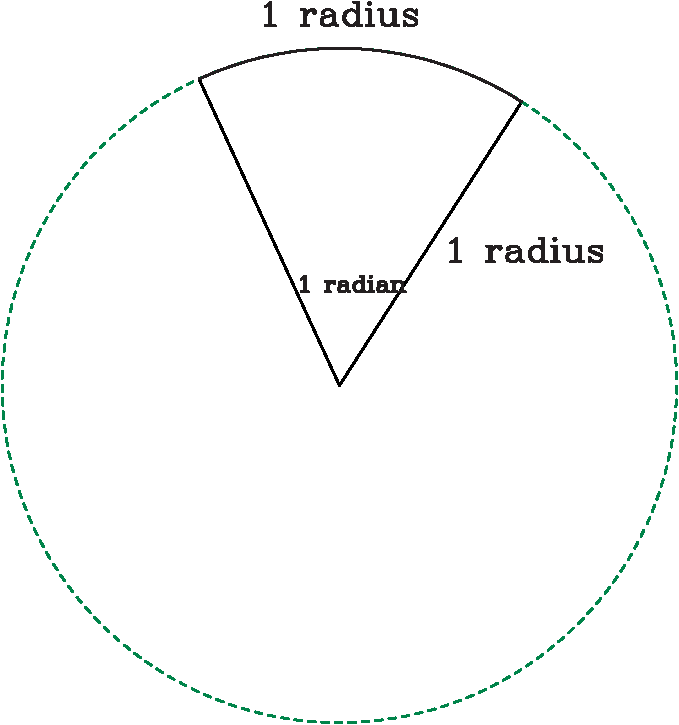
\includegraphics[width=0.30\textwidth]{circle1-crop.pdf}\hspace{0.15\textwidth}
  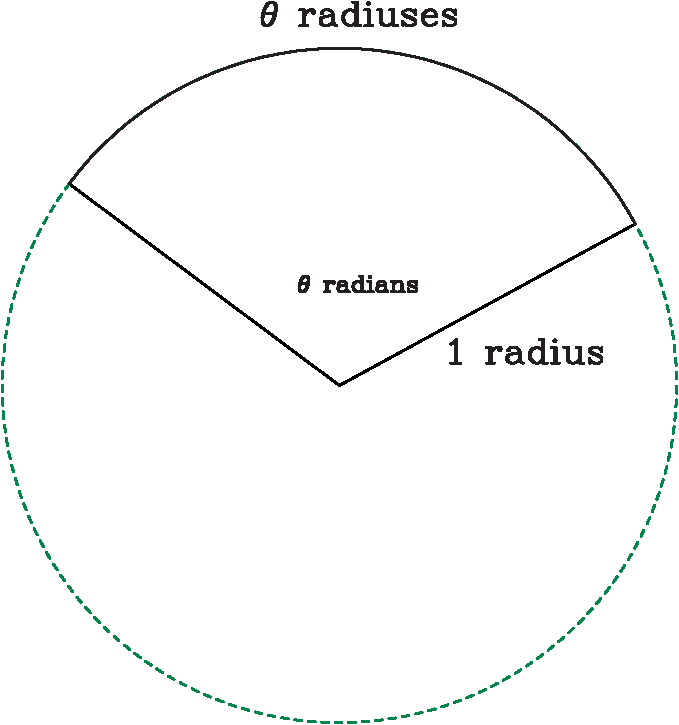
\includegraphics[width=0.30\textwidth]{circle2-crop.pdf}

\bigskip

  \centerline{\color{Red}$\rightarrow$ Tangential movement (in meters) = angular movement (in radians) times the radius}
}


\frame{\frametitle{\textbf{Rotational motion: description}}
  \Large Some new terms:
  \large
  \begin{itemize}
    \item{``Radial'': directed in and out of the circle}
    \item{``Tangential'': directed around the circle}
    \item{The radial velocity is 0 ($r$ doesn't change)}
    \item{The tangential velocity depends on $r$ and $\omega$, as you'd expect}
      \pause
    \item{$v_T = \omega r$: ``meters per second = radians per second times meters per radian''}
  \end{itemize}
}


\frame{

\Large
Which way is the object on the string accelerating at the top of the arc?

\bigskip
\bigskip


\color{A}A: Upward: it is at the top of the arc, and it must have accelerated upward to get there \\
\bigskip

\color{B}B: Upward: its upward acceleration is what keeps the string taut at the top of the swing\\ 
\bigskip

\color{C}C: Downward: the only forces acting on it there pull it downward, so by $\vec F=m\vec a$ it must be accelerating downward \\
\bigskip

\color{D}D: Downward: it was moving up and to the left, then down and to the left, so the net change is ``down'' \\
\bigskip

\color{E}E: Zero: it is being swung at a constant rate
} 



\frame{\frametitle{\textbf{Kinematic challenge: what's $\vec a$?}}
\Large

Clearly an object moving in a circle is accelerating. What's the acceleration?

  \hspace{0.1\textwidth}
  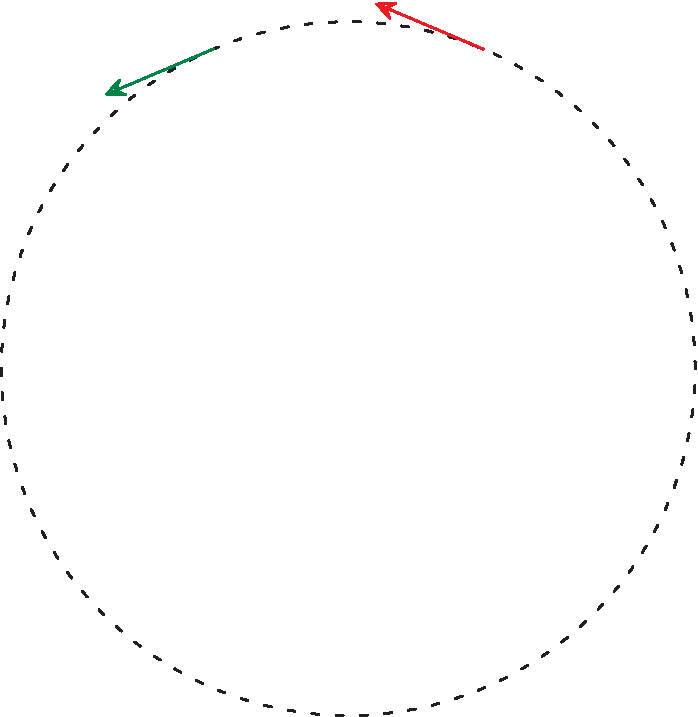
\includegraphics[width=0.30\textwidth]{acc1-crop.pdf}\hspace{0.15\textwidth}
  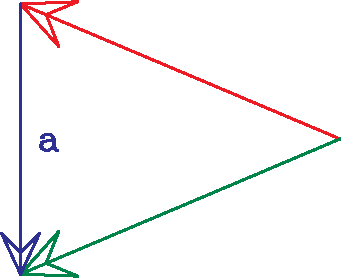
\includegraphics[width=0.30\textwidth]{acc2-crop.pdf}


\bigskip
  
  \large
\pause

Near the top of the circle, the $y$-component of the velocity decreases; we expect then that $\vec a$ points downward.

\bigskip

Can we make this rigorous?

}


\frame{\frametitle{\textbf{Some math}}
\large

$x(t) = r \cos (\omega t)$

$y(t) = r \sin (\omega t)$

\pause

\bigskip
\bigskip

Differentiate to get $v_x$ and $v_y$:

\bigskip

$v_x(t) = -\omega r \sin (\omega t)$

$v_y(t) = \,\,\,\,\omega r \cos (\omega t)$

\pause

\bigskip
\bigskip

Differentiate again to get $a_x$ and $a_y$:

\bigskip

$a_x(t) = -\omega^2 r \cos (\omega t) = -\omega^2 x(t)$

$a_y(t) = -\omega^2 r \sin (\omega t) = -\omega^2 y(t)$

\pause

\bigskip
\bigskip

$\rightarrow \vec a = -\omega^2 \vec r$

\bigskip
\pause

{\color{Red}An object in uniform circular motion accelerates toward the center of the circle with }

\bigskip

\centerline{  \color{Green}$\rightarrow a=\omega^2 r=v^2/r \leftarrow $}
}

\frame{\frametitle{\textbf{Uniform circular motion, consequences}}
  \large
  If you know an object is undergoing uniform circular motion, you know something about the acceleration:

\bigskip

\centerline{\color{Red} $a=\omega^2 r$ or $a=v^2/r$ toward the center of the circle.}

\bigskip

\pause

Circular motion problems aren't scary; they are just like any other force problem.

\begin{itemize}
  \item{Equilibrium problem: $\sum F_x = ma_x = 0$ and $\sum F_y = ma_y = 0$}
  \item{Circular motion problem: $\sum F_T = ma_T = 0$ and $\sum F_r = ma_r = v^2/r$}
  \end{itemize}

  \bigskip

  $\rightarrow$ If we tell you that a thing is in uniform circular motion, we're just telling you something about its acceleration.

}

\frame{

\Large

Of all of the topics in Physics 211, this is the one topic that students overcomplicate the most.

\bigskip

Circular motion problems are {\it just like any other} Newton's-law problem. The only difference is that
you know something about the object's acceleration. Do not make these more complicated than they actually
are!
}


\frame{\frametitle{\textbf{Forces toward the center}}
  \large
  ``Centripetal'' means ``toward the center'' in Latin.
  
  \bigskip\bigskip
  
  If something moves in a circle, it is accelerating toward the center at $a = \omega^2 r$.

\bigskip
\BI
\item{If something is going to accelerate toward the center, a force must do that.}

\item{Centripetal force is {\color{Red} not} a ``new'' force. No arrows labeled ``centripetal force''!}

\item{``Centripetal'' is a word that describes a force you already know about.}
\item{Centripetal force: describes a force that holds something in a circle}


\item{It can be lots of things:}
  \BI
  \normalsize
\item{Tension (see our demos)}
\item{Normal force (platform, bucket demos)}
\item{Friction (Ferris wheel)}
\item{Gravity (the moon!)}
  \EI
  \EI
}


\frame{
\large
What does the force diagram on the water look like while the bucket is at the bottom?

\BI
\item{\color{A}A: acceleration upward, normal force upward, gravity downward}
\item{\color{B}B: centripetal force upward, normal force upward, gravity downward}
\item{\color{C}C: gravity downward, normal force upward}
\item{\color{D}D: gravity downward, velocity to the left, normal force upward}
\EI
}

\frame{
\large
Why doesn't the water in the bucket fall at the top?

\BI
\item{\color{A}A: It {\it is} falling, but the bucket falls along with it, so it stays in}
\item{\color{B}B: The normal force pushes it up} 
\item{\color{C}C: The centripetal force pushes it up}
\pause
\item{\color{D}D: Sam is in the back chanting ``wingardium leviosa!''}
\EI
}

\frame{
\large
What does the force diagram on the water look like while the bucket is at the top?

\BI
\item{\color{A}A: acceleration downward, normal force upward, gravity downward}
\item{\color{B}B: normal force upward, gravity downward}
\item{\color{C}C: gravity downward, normal force downward}
\item{\color{D}D: normal force downward, gravity downward, centrifugal force upward} 
\EI
}


\frame{
\large
What is the acceleration of the water at the top?

\BI
\item{\color{A}A: Zero}
\item{\color{B}B: Downward, less than $g$ }
\item{\color{C}C: Downward, equal to $g$} 
\item{\color{D}D: Downward, more than $g$}
\item{\color{E}E: Upward} 
\EI
}


\frame{
	\large
	What is the tension in the string at the bottom?
	
	\BI
	\item{\color{A}A: $mg + m\omega^2 r$}
	\item{\color{B}B: $mg$ }
	\item{\color{C}C: $mg - m \omega^2 r$} 
	\item{\color{D}D: $m \omega^2 r$}
	\item{\color{E}E: $m \omega^2 r - mg$} 
	\EI
}


\frame{
	\large
	What is the tension in the string at the top?
	
	\BI
	\item{\color{A}A: $mg + m\omega^2 r$}
	\item{\color{B}B: $mg$ }
	\item{\color{C}C: $mg - m \omega^2 r$} 
	\item{\color{D}D: $m \omega^2 r$}
	\item{\color{E}E: $m \omega^2 r - mg$} 
	\EI
}




\frame{\frametitle{\textbf{Driving around a road curve}}
	What is the fastest I can drive around a flat interstate on-ramp? What if it is snowy? What if it is icy?
}


%\frame{\frametitle{\textbf{Sample problems}}
%\large
%Suppose we get a standard-issue physics frog and put him in the bucket. We reassure him that we won't drop him,
%so he won't hop out; our frogs are confident that we can do physics.
%
%\bigskip
%
%Suppose that my arm has a length $L$, and that the frog has a mass $m$. What's the minimum speed $v$
%that I must swing the bucket so that the frog doesn't fall out? 
%
%\bigskip
%
%\BI
%\item{\color{A}A: $\omega^2 L$}
%\item{\color{B}B: $gL$} 
%\item{\color{C}C: $\sqrt{2gL} $}
%\item{\color{D}D: $\sqrt{gL}$}
%\EI
%}
%
%
%\frame{\frametitle{\textbf{Sample problems}}
%\large
%Suppose we get a standard-issue physics frog and put him in the bucket. We reassure him that we won't drop him,
%so he won't hop out; our frogs are confident that we can do physics.
%
%\bigskip
%
%Suppose that my arm has a length $L$, and that the frog has a mass $m$; suppose I'm swinging my arm at
%an angular velocity $\omega$. What is the frog's apparent weight
%at the bottom of the circle? 
%
%\bigskip
%
%\BI
%\item{\color{A}A: $mg$}
%\item{\color{B}B: $mg-\omega^2 L$} 
%\item{\color{C}C: $mg+\omega^2 L$}
%\item{\color{D}D: $2mg$}
%\EI
%}






\end{document}
